\documentclass{beamer}

\usepackage{graphicx,hyperref,udesc,url}
\usepackage[latin1]{inputenc}
\usepackage{bussproofs}
%\usepackage[T1]{fontenc}
\usepackage{booktabs}
\usepackage[portuges]{babel}

\AtBeginSection[]{
  \begin{frame}[noframenumbering]
  \vfill
  \centering
  \begin{beamercolorbox}[sep=8pt,center,shadow=true,rounded=true]{title}
    \usebeamerfont{title}\insertsectionhead\par%
  \end{beamercolorbox}
  \vfill
  \end{frame}
}

\AtBeginSubsection[]{
  \begin{frame}[noframenumbering]
  \vfill
  \centering
  \begin{beamercolorbox}[sep=8pt,center,shadow=true,rounded=true]{title}
    \usebeamerfont{title}\insertsubsectionhead\par%
  \end{beamercolorbox}
  \vfill
  \end{frame}
}
\newcommand\Wider[2][3em]{%
\makebox[\linewidth][c]{%
  \begin{minipage}{\dimexpr\textwidth+#1\relax}
  \raggedright#2
  \end{minipage}%
  }%
}

\title[Extraction of Programs from Proofs]{Programming = Mathematics + Murphy's Law\\ - (E. Dijkstra)}

\author[Rafael Castro, Karina Roggia]{
    Rafael Castro\\\medskip
    {\small \url{rafaelcgs10@gmail.com}}\\\medskip
    Karina Roggia\\\medskip
    {\small \url{karina.roggia@udesc.br}}
  }

\date{04/09/2019}

\begin{document}

\begin{frame}
  \titlepage

\end{frame}

\section{Mini-bibliografia}

\begin{frame}
  \frametitle{Quem foi Edsger Dijkstra?}
  \begin{columns}
    \begin{column}{.555555\textwidth}
      \begin{itemize}
      \item Nome Completo: Edsger Wybe Dijkstra.
      \item Nacionalidade: Holand�s.
      \item Longevidade: 1930 - 2002.
      \end{itemize}
    \end{column}
    \begin{column}{.555555\textwidth}
      \begin{figure}
        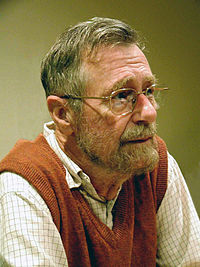
\includegraphics[width = 0.7\textwidth]{dijkstra.jpg}
      \end{figure}
    \end{column}
  \end{columns}
\end{frame}

\begin{frame}
  \frametitle{Alguns trabalhos de Edsger Dijkstra}
  \begin{itemize}
  \item Algoritmos de grafos: Prim e Dijkstra.
  \item Sistema Operacional THE (BATCH, camadas de abstra��o e multitasking).
  \item Vari�vel de sem�foro.
  \item Trabalhou no primeiro compilador da linguagem ALGOL 60.
  \item Introduziu o conceito de pilha em programas recursivos.
  \item Pai da programa��o estruturada - Uso de subrotinas, la�os de repeti��o etc.
  \item Defensor do uso de metodologias matem�ticas na programa��o - Verifica��o formal.
  \item Escreveu diversos textos (EWDs).
  \end{itemize}
\end{frame}

\begin{frame}
  \frametitle{Pr�mios que Dijkstra ganhou}
  \begin{enumerate}
  \item Fellow da British Computer Society em 1971.
  \item Membro da Royal Netherlands Academy of Arts and Sciences em 1971.
  \item ACM Turing Award em 1972.
  \item American Academy of Arts and Sciences em 1975.
  \item Fellow da Association for Computing Machinery 1994.
  \end{enumerate}
\end{frame}

\section{Frases de Dijkstra}

\begin{frame}
  \frametitle{Divis�o}
  \begin{itemize}
  \item Frases que todos citam, mas que ningu�m sabe o contexto
  \item Frases falando mal de Engenharia de Software
  \item Frases falando mal de Ensino de C. da Computa��o
  \item Frases falando mal de linguagens de programa��o
  \end{itemize}
\end{frame}

\subsection{Frases que todos citam, mas que ningu�m sabe o contexto}

\begin{frame}
  \frametitle{Ci�ncia da Computa��o � sobre ...}
  \centering
  \includegraphics[width = 0.7\textwidth]{computer-science-is-.jpg}
  \pause
  \\
  \Large{N�o � do Dijkstra!}
  \pause
  \\
  Michael R. Fellows, Ian Parberry (1993) "SIGACT trying to get children excited about CS"
\end{frame}


\begin{frame}
  \frametitle{Simplicidade � uma grande virtude...}
  \begin{figure}
    \centering
    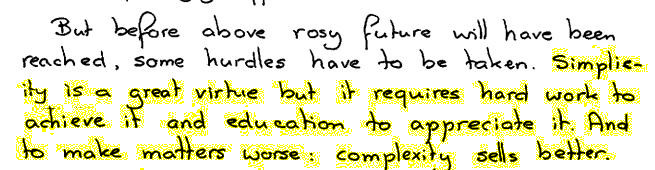
\includegraphics[width = 1.0\textwidth]{896.jpeg}
  \end{figure}
  \begin{small}
  \begin{itemize}
    \item EWD 896 - 10 de Agosto de 1984
    \item O texto questiona a natureza da Ci�ncia da Computa��o.
    \item Contexto: ``a computa��o vai curar todos os males do mundo'' - a busca pela Pedra Filosofal.
    \item Como a computa��o se afirma como uma disciplina acad�mica?\\ Atrav�s da matem�tica.
    \item Se � simples, n�o � relevante: rejeitaram um artigo do Dijkstra porque a solu��o era muito simples.
  \end{itemize}
  \end{small}
\end{frame}


\end{document}
%%% Local Variables:
%%% mode: latex
%%% TeX-master: t
%%% End:
